\begin{frame}{Retrieval or a Longer Window}
  Retrieval-augmented generation is a long-standing way around a short window. Two studies a year apart compared it with reading the whole input.
  \vspace{0.4em}
  \begin{columns}[T,onlytextwidth]
    \column{0.49\textwidth}
      \textbf{2023: Llama2-70B and a 43B GPT}
      \begin{itemize}\footnotesize\itemsep0.3em
        \item[\textcolor{red}{$\blacktriangleright$}] A 4K window plus retrieval matched a window extended to 16K by position interpolation: average 36.02 vs 36.78 (Llama2-70B) and 29.32 vs 29.45 (GPT-43B), with much less computation.
        \item[\textcolor{red}{$\blacktriangleright$}] Retrieval still helped the long model: Llama2-70B-32k scored 40.9 without it and 43.6 with it, above GPT-3.5-turbo-16k (42.8), and generated 4$\times$ faster on NarrativeQA.
      \end{itemize}
    \column{0.49\textwidth}
      \textbf{2024: Gemini-1.5-Pro, GPT-4o, GPT-3.5-Turbo}
      \begin{itemize}\footnotesize\itemsep0.3em
        \item[\textcolor{red}{$\blacktriangleright$}] With enough resources, the long-context (LC) model beat retrieval on average: 49.70 vs 37.33 for Gemini-1.5-Pro and 48.67 vs 32.60 for GPT-4o.
        \item[\textcolor{red}{$\blacktriangleright$}] Retrieval cost 17\% of the long-context run, and for 63\% of queries the two setups gave identical predictions, right and wrong alike.
      \end{itemize}
  \end{columns}
  \vspace{0.5em}
  \begin{itemize}\footnotesize
    \item[\textcolor{red}{$\blacktriangleright$}] The verdict moved because models got better at using long inputs. The cost gap did not move: most queries can be answered from a few retrieved chunks.
  \end{itemize}
  \vspace{0.2em}
  {\scriptsize Xu et al., ``Retrieval Meets Long Context Large Language Models,'' ICLR 2024, \href{https://arxiv.org/abs/2310.03025v2}{arXiv:2310.03025v2}, Section~1. Li et al., ``Retrieval Augmented Generation or Long-Context LLMs? A Comprehensive Study and Hybrid Approach,'' EMNLP 2024 Industry Track, \href{https://arxiv.org/abs/2407.16833v2}{arXiv:2407.16833v2}, Figure~1, Table~1 and Section~4.1.}
\end{frame}

\begin{frame}{Self-Route: Let the Model Decide}
  \begin{columns}[T,onlytextwidth]
    \column{0.46\textwidth}
      \begin{itemize}\footnotesize\itemsep0.4em
        \item[\textcolor{red}{$\blacktriangleright$}] \textbf{Step 1, retrieve and route.} Give the model the query and the retrieved chunks (about 1.5k tokens) and allow it to reply ``unanswerable''. Answerable queries stop here.
        \item[\textcolor{red}{$\blacktriangleright$}] \textbf{Step 2, read everything.} Only the queries declared unanswerable go to the long-context model with the full input (10k to 100k tokens).
        \item[\textcolor{red}{$\blacktriangleright$}] The router is the model's own judgment of whether the chunks suffice, so no extra classifier is trained.
        \item[\textcolor{red}{$\blacktriangleright$}] Self-Route used 38\% of the long-context cost with Gemini-1.5-Pro and 61\% with GPT-4o, at average scores close to the long-context model (46.41 vs 49.70 and 48.89 vs 48.67).
      \end{itemize}
    \column{0.52\textwidth}
      \centering
      \vspace{0.2em}
      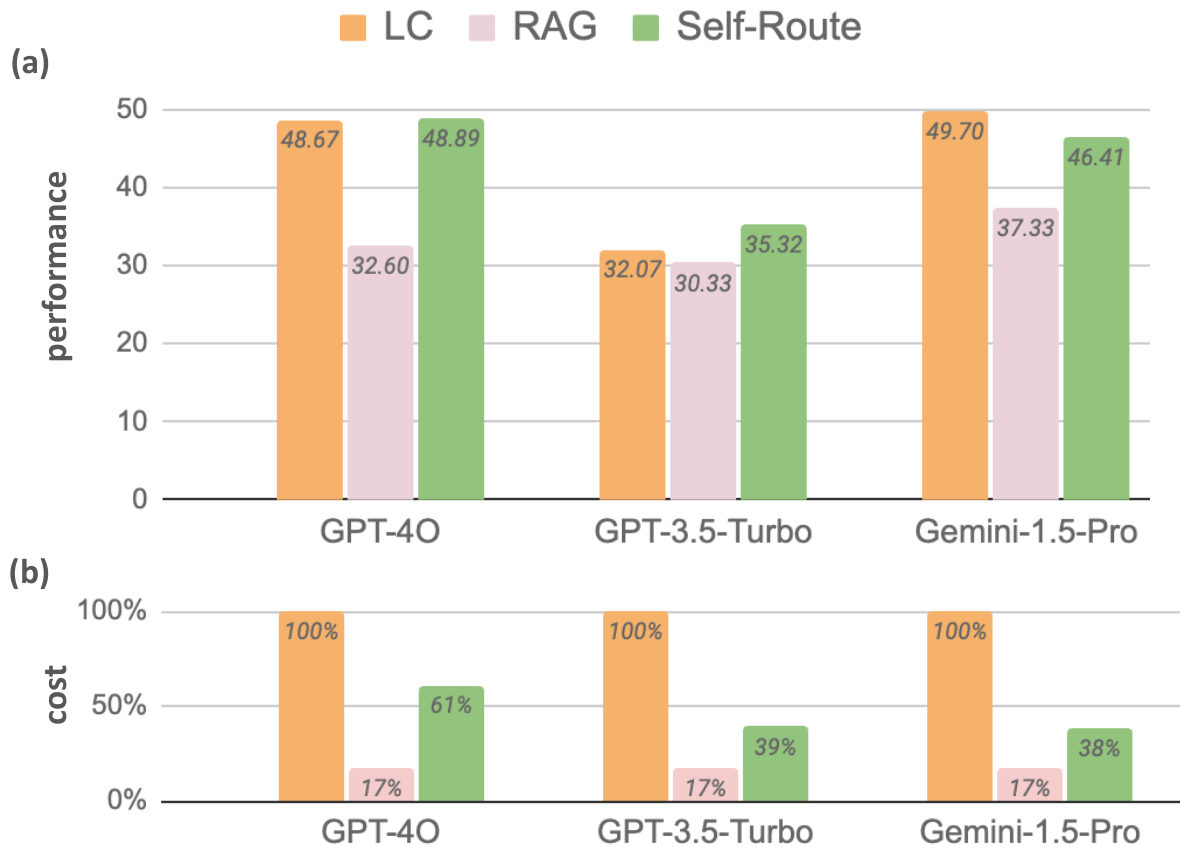
\includegraphics[width=\linewidth,height=0.62\textheight,keepaspectratio]{images/long-context/selfroute_fig1_lc_rag_selfroute_cost.png}\\[0.2em]
      {\scriptsize ``While long-context LLMs (LC) surpass RAG in long-context understanding, RAG is significantly more cost-efficient.'' Li et al., \href{https://arxiv.org/abs/2407.16833v2}{arXiv:2407.16833v2}, Figure~1.}
  \end{columns}
\end{frame}

\begin{frame}{The Families Side by Side}
  \centering
  {\scriptsize
  \begin{tabular}{>{\raggedright\arraybackslash}p{2.5cm} >{\raggedright\arraybackslash}p{2.1cm} >{\raggedright\arraybackslash}p{2.4cm} >{\raggedright\arraybackslash}p{2.0cm} >{\raggedright\arraybackslash}p{2.7cm}}
    \toprule
    \textbf{Family} & \textbf{What shrinks} & \textbf{Exact recall of an old token} & \textbf{Training} & \textbf{Typical failure} \\
    \midrule
    Hard prompt compression & tokens read & no, once dropped & small compressor & numbers and names dropped \\
    \addlinespace[0.15em]
    Soft compression & tokens become vectors & approximate & encoder or LLM fine-tune & exact strings blur \\
    \addlinespace[0.15em]
    KV-cache eviction & cache to $B$ entries & no, once evicted & none & needle evicted before the question \\
    \addlinespace[0.15em]
    Fixed sparse patterns & $n^2$ to about $n\,w$ & through global tokens and depth & pretraining or adaptation & pattern ignores content \\
    \addlinespace[0.15em]
    Learned block selection & $n^2$ to about $n^2/b + n\,k\,b$ & yes, if its block is chosen & native or continued training & selection misses \\
    \addlinespace[0.15em]
    Segment recurrence & memory per segment & no, beyond the memory & training through segments & sequential, slower training \\
    \addlinespace[0.15em]
    Linear-attention memory & a fixed-size state & no, capacity bound & pretraining & recall-heavy tasks \\
    \addlinespace[0.15em]
    Retrieval & tokens read & only what is retrieved & a retriever & retrieval misses, multi-hop \\
    \bottomrule
  \end{tabular}\par}
  \vspace{0.6em}
  \begin{itemize}\footnotesize
    \item[\textcolor{red}{$\blacktriangleright$}] Production systems combine rows: sparse or linear layers for most of the depth, a few full-attention layers for exact recall, quantized caches, and retrieval in front.
  \end{itemize}
\end{frame}

\begin{frame}{A Decision Guide}
  \begin{enumerate}\footnotesize\itemsep0.45em
    \item \textbf{Measure first.} Probe the model at your real input lengths with RULER- or NoLiMa-style tasks built from your own data. The effective length bounds what any later technique can deliver, whatever the advertised window.
    \item \textbf{Knowledge in a large or changing corpus:} retrieve, and send the full context only when the retrieved chunks cannot answer, as Self-Route does.
    \item \textbf{One long document that must be read whole, with serving memory as the limit:} compress the cache with quantization and query-aware eviction. Keep the full prompt when follow-up questions are unknown in advance.
    \item \textbf{An unbounded stream:} sink tokens plus a recent window keep generation fluent; add a recurrent memory when old content must be recalled.
    \item \textbf{Training a model:} build length in with block-sparse attention or delta-rule layers, mixed with a few full-attention layers.
    \item \textbf{Re-measure after every change} on the same probe. Compression and sparsity fail silently, and they fail first on the long-range cases.
  \end{enumerate}
\end{frame}
